\chapter{Results}

The experiments were performed in a Dell XPS 15 9575, with a $4.1$GHz Intel Core i7-80705G CPU and $16$GB of RAM, plus $8$GB of SSD swap. 

\section{The \dBCM as a \dBG representation}
\label{sec:results-dbcm-counting}

To assess how well the \dBCM can represent a \dBG when constructed from the raw sequencing reads, we first analyze how accurately it performs \kmer counting. We constructed a set of \dBCM instances with varying dimensions $w \in \{7.5\text{M}, 10\text{M}, \ldots 17.5\text{M}, 20\text{M}\}$\footnote{$1\mega = 10^6$} and $d \in \{6, 8\}$ from a set of synthetic reads generated from the \emph{E.~Coli} reference genome \cite{ecoligenome} using the \emph{ART Illumina} simulation toolkit \cite{Huang2011} with a coverage $c=80\times$. For each instance, we calculated the mean and standard deviation of the individual count errors $\Delta(X) = C.\mathit{query}(X) - c(X)$. In Figure~\ref{fig:ecoli-art-dbcm-errors} we plot these two metrics as a function of $w$ for the two values of $d$.

\begin{figure}[htb]
    \centering
    \begin{subfigure}{.5\textwidth}
        \centering
        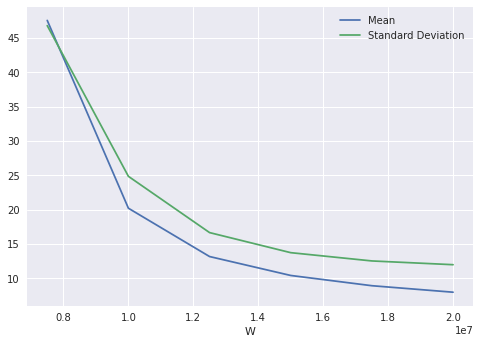
\includegraphics[width=\textwidth]{figures/e_coli-error_mean_stddev-K31-D6-T40}
        \caption{$d = 6$}\label{fig:ecoli-art-dbcm-errors-d6}
    \end{subfigure}%
    \begin{subfigure}{.5\textwidth}
        \centering
        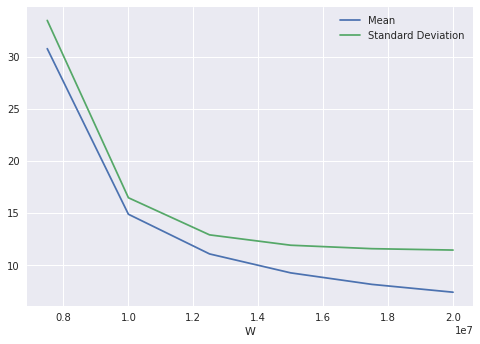
\includegraphics[width=\textwidth]{figures/e_coli-error_mean_stddev-K31-D8-T40}
        \caption{$d = 8$}\label{fig:ecoli-art-dbcm-errors-d8}
    \end{subfigure}
	\caption{\dBCM miscount mean and standard deviation as a function of $w$ for $d = 6$ and $d = 8$}\label{fig:ecoli-art-dbcm-errors}
\end{figure}

We observe only a slight improvement in the overestimation error mean and standard deviation for for $w\geq 10\mega$. However, we are not so much interested in the absolute counts per se, but rather as way of discerning real \kmers occurring in original sequence from spurious \kmers appearing only in the reads due to sequencing errors. In order to save memory, we would like to use the smallest values allowing for this separation.
To check whether the \dBCM can effectively differentiate between these two categories, we select $w=10\mega$ and $d=6$ and compare the distribution of the count estimates with the actual values for the \kmer{s} in the reads. This comparison can be observed in Figure~\ref{fig:ecoli-art-dbcm-counts}. \toconsider{Note that, in the exact count distribution, close to $9\mega$ \kmer{s} have frequency between $2^4$ and $2^6$. This matches the expected number of real \kmer{s} from the sequence in forward and reverse complement forms.} \paguso{seria bom indicar a quantidade de \kmers nas barrinhas pequenas da contagem exata. esse numero deveria ser próximo do número real de \kmers na sequência pra gente poder argumentar que os \kmers reais são os que têm alta frequência} Although the estimated counts distribution is shifted right due to overcount, we see two peaks, one between $2^3$ and $2^4$, and the other between $2^6$ and $2^7$, indicating the high- and low-frequency categories may still be discernible although a threshold is not as clear as with the exact counts.
Combining these observations, we see that for $w \geq 10\mega$, both error mean and standard deviation are below $30$ regardless of $d$, such that we expect over $80\%$\paguso{de onde vem esse 80\%?}, of spurious \kmer{s} to have a count no greater than $60$, while real \kmer{s} are expected to have a count not much lower than $80$ (the coverage). This suggests that high- and low-frequency \kmer{s} are likely to still be discernible based on a threshold in the 30--60 range.


\begin{figure}[htb]
    \centering
    \begin{subfigure}{.5\textwidth}
        \centering
        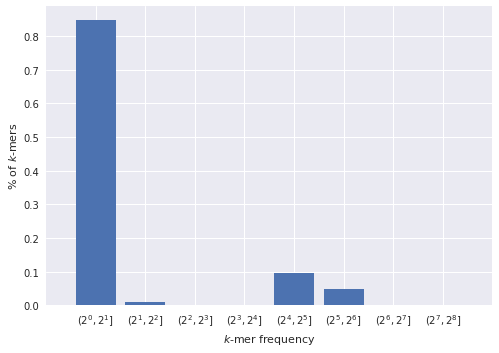
\includegraphics[width=\textwidth]{figures/e_coli-kmer_frequencies-exact-K31}
        \caption{Exact}\label{fig:ecoli-art-dbcm-counts-exact}
    \end{subfigure}%
    \begin{subfigure}{.5\textwidth}
        \centering
        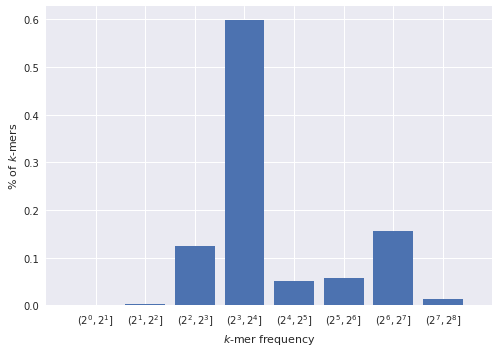
\includegraphics[width=\textwidth]{figures/e_coli-kmer_frequencies-estimated-K31-W10000000-D6}
        \caption{Estimated ($w = 10\mega, d = 6$)}\label{fig:ecoli-art-dbcm-counts-exact}
    \end{subfigure}
	\caption{\kmer count distribution}\label{fig:ecoli-art-dbcm-counts}
\end{figure}

Next we evaluate possible thresholds $t$ in the range $[1, 2c]$ by analyzing the \keyterm{true positive rate}, or \keyterm{sensitivity}, of the \dBCM, i.e. percentage of true \kmer{s} correctly identified, as well as its \keyterm{false positive rate}, i.e. percentage of false \kmer{s} erroneously identified as true, using each one of those values. The results are presented in Figure~\ref{fig:ecoli-art-dbcm-threshold-estimated}, where we can see that, without excluding any true \kmer{s} from the \dBG, we can filter out over $80\%$ of the spurious \kmer{s} from the reads by using $20 \leq t \leq 40$. However, comparing these results with the sensitivity and false positive rate if using the exact counts (Figure~\ref{fig:ecoli-art-dbcm-threshold-exact}), we can see that the number of false positives nearly doubles when keeping sensitivity maximized. In the synthetic reads dataset used, this equates to nearly $9.7\mega$ spurious \kmer{s} being added to the \dBG, over $5\mega$ more than would be added using exact counts. In the following section we show that, despite this increase in number of spurious \kmer{s} represented in the \dBCM, only a fraction of them are reachable in traversal, such that this representation still succeeds in filtering out erroneous \kmer{s}.

A \dBCM with $w = 10\mega$ and $d = 6$ needs $16 \times 10\mega \times 6 = 960\mega$ bits, or $120$MB. The time needed for construction of the \dBCM is linear on the total number of bases in the reads, and took $6$ minutes in the experimental environment.

\begin{figure}[htbp]
    \centering
    \begin{subfigure}{.5\textwidth}
        \centering
        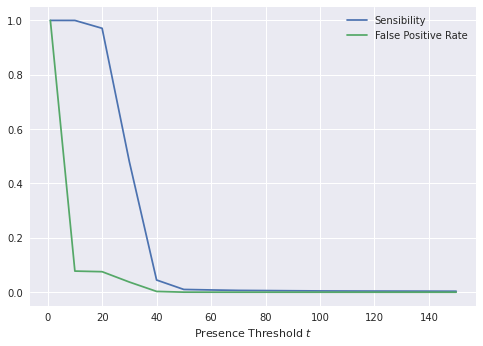
\includegraphics[width=\textwidth]{figures/e_coli-threshold_exploration-K31-exact}
        \caption{Exact counts}\label{fig:ecoli-art-dbcm-threshold-exact}
    \end{subfigure}%
    \begin{subfigure}{.5\textwidth}
        \centering
        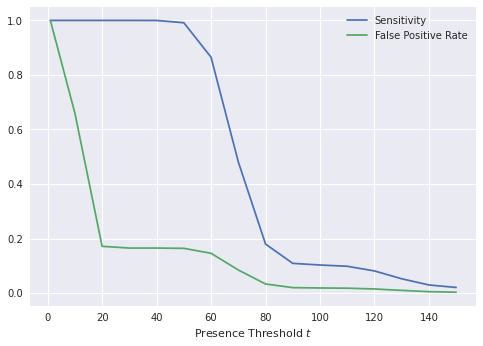
\includegraphics[width=\textwidth]{figures/e_coli-threshold_exploration-K31-W10000000-D6}
        \caption{Estimated by \dBCM ($w=10\mega, d=6$)}\label{fig:ecoli-art-dbcm-threshold-estimated}
    \end{subfigure}
    \caption{Sensitivity and False Positive Rate of a \dBCM with $w = 10\mega$ and $d = 6$ as a function of the presence threshold $t$}\label{fig:ecoli-art-dbcm-threshold}
\end{figure}

\section{Filtering through traversal}
\label{sec:results-dbcm-traversal}

As discussed in Section~\ref{sec:pipeline}, we expect many of the spurious \kmer{s} inserted into the \dBG due to high frequency to be disconnected from the main component of the graph, containing the real \kmer{s}. By traversing the graph from a small sample of these high-frequency \kmer{s}, we expect never to visit most of these disconnected components, such that using the set of \kmer{s} visited during traversal, rather than the set of high-frequency \kmer{s}, to construct a representation of the \dBG should lead to fewer distinct \kmer{s} inserted into the graph, allowing for a more succint representation.

To evaluate this claim, we construct a \dBCM with $w = 10\mega$, $d = 6$, and using $t = 40$, from the unprocessed set of synthetic reads used in Section~\ref{sec:results-dbcm-counting}. We then traverse the graph from a subset of high-frequency \kmer{s} found at the start of the reads, logging the \kmer{s} that were queried and their query results. Afterwards, we counted the number of queried \kmer{s} to be $\approx 9.62\mega$, as well as the number of those that were visited $\approx 9.58\mega$. Of those visited, only $173\kilo$ were not found in the original DNA sequence in either forward or reverse complement form, approximately $1.8\%$ of the number of spurious \kmer{s} that would be added, from the reads, into a \dBG based on the count estimated by the same \dBCM, and $3.8\%$ of the spurious \kmer{s} from the reads that would be added based on their true counts. In a hashtable-based representation, as the \dBHT, this would reduce the number of cells needed by \emph{one third} when compared with using the exact counts as the requirement for insertion.

Traversing the \dBCM was done in around $30$ seconds when the queried \kmer{s} were not being logged to an output file, and twice that when writing to disk.\asq{Eu acho que esse resultado de tempo é meio inutilizável, porque eu usei um set em memória dos \kmer{s} visitados, de forma que isso não é escalável para genomas maiores. Não só a travessia, do jeito que está implementada agora, seria impossível sem uma quantidade enorme de memória, como ela acabaria usando uma representação não-sucinta do \dBG para ser capaz de dizer se um \kmer foi visitado ou não. Seria necessário fazer a travessia usando do disco, ou usar alguma outra estrutura sucinta através da qual pudessemos identificar quais \kmer{s} foram visitados. No final das contas talvez acabe não fazendo sentido? O mesmo vale para a travessia da dBHT}

\section{\dBHT as a NDS representing a \dBG}
\label{sec:results-dbht}

Finally, we want to evaluate how different the graph represented by the \dBHT is to the graph represented by the \dBCM, from which it was generated. Although the \dBHT is a probabilistic representation, note that a node inserted into it is always found when queried, likewise for outedges, such that there should be no loss in sensitivity when going from one representation to the other. Where the \dBHT may introduce error is when collisions occur. Because, the \kmer is not directly represented in the hashtable, only its fingerprint, two \kmer{s} can be mapped to the same cell. This can incur in \kmer{s} sharing the set of outedges which, in turn, can incur in false \kmer{s} being queried and found, again through collision. The chance of collision\asq{collision collision}, however, is controled by the choice of load factor $\alpha$. Therefore, we evaluate the traversal performance of \dBHT{s} with varying load factors $\alpha \in \{0.5, 0.55, \ldots, 0.85, 0.9\}$ constructed from a traversal of the \dBCM with $w = 10\mega$, $d = 6$, and using $t = 40$. \asq{dois ``traversal'' na mesma frase. Talvez a essa altura eu possa suprimir o segundo traversal, uma vez que já foi deixado claro que construir uma \dBHT de um \dBCM é através do traversal}

In Figure~\ref{fig:ecoli-art-dbht-traversal-queryfound}, we can see that the number of \kmer{s} queried during traversal, and \tochange{XXX} the number of \kmer{s} visited, grows with $\alpha$, as the table size shrinks and collisions become more common. This results naturally results in a growth of in the number of false positives, as evidenced in Figure~\ref{fig:ecoli-art-dbht-traversal-positives}. Note that, even in the best case observed, when $\alpha = 0.5$, the number of false positives, $348\kilo$ \kmer{s}, is still greater than the value observed in traversal of the \dBCM by a factor of $2$. It is, however, much less than the number of false \kmer{s} that would be \emph{explicitly} inserted into the \dBHT based on count alone, even exact. Figure~\ref{fig:ecoli-art-dbht-traversal-sensitivity} confirms that there is no loss in sensitivity from going from the \dBCM representation to the \dBHT.

\begin{figure}[htbp]
    \centering
    \begin{subfigure}{.5\textwidth}
        \centering
        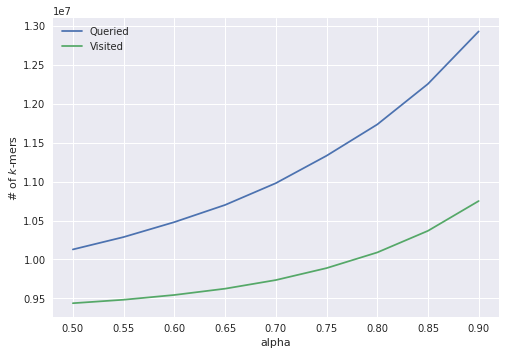
\includegraphics[width=\textwidth]{figures/e_coli-dbht-queried_and_found}
        \caption{Number of \kmer{s} queried (blue) and visited (green)}\label{fig:ecoli-art-dbht-traversal-queryfound}
    \end{subfigure}
    \begin{subfigure}{.5\textwidth}
        \centering
        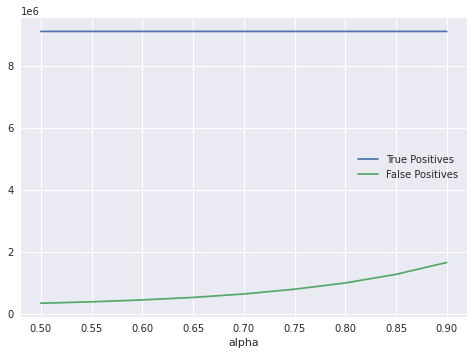
\includegraphics[width=\textwidth]{figures/e_coli-dbht-true_and_false_positive_counts}
        \caption{True (blue) and false (green) positive counts}\label{fig:ecoli-art-dbht-traversal-positives}
    \end{subfigure}%
    \begin{subfigure}{.5\textwidth}
        \centering
        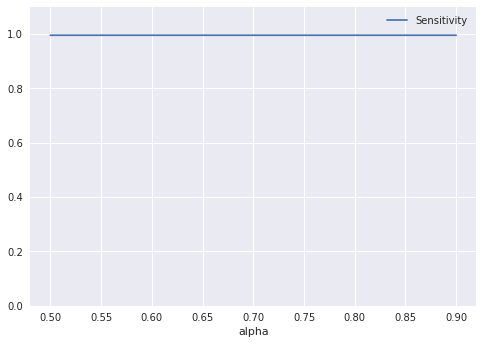
\includegraphics[width=\textwidth]{figures/e_coli-dbht-sensitivity}
        \caption{Sensitivity}\label{fig:ecoli-art-dbht-traversal-sensitivity}
    \end{subfigure}
    \caption{Traversal results for \dBHT according to load factor $\alpha$}\label{fig:ecoli-art-dbcm-threshold}
\end{figure}